\documentclass[12pt]{article}
\usepackage{graphicx}
\usepackage[german]{babel}
\usepackage{url}
\usepackage{fontspec}

\begin{document}

\title{Gestensteuerung mithilfe Künstlicher Intelligenz}
\date{28. Januar, 2020}
\author{Silvan Metzker, Projektunterricht, Leitung: Patric Rousselot}
\maketitle
\newpage
\tableofcontents
\newpage

\section{Vorwort}
Die Idee für ein solches Projekt kam mir während einer Diskussion mit meinem Vater in den Ferien. Mein Vater arbeitet bei einem Hausgeräte-Hersteller und erzählte mir über die Idee von Küchengeräten, welche durch eine Kochapp gesteuert werden. Auch erzählte er mir von einem Wegesystem im Kochherd, welche mithilfe des Gewichtes der Kochapp sagt, wie viele Gramm einer Zutat noch fehlen. Ich hatte damals schon immer die Absicht, etwas mithilfe von Künstlicher Intelligenz, kurz KI, zu analysieren. So kam mir damals die Idee einer App, welche mithilfe Gesten gesteuert wird.

\section{Einleitung}
Stellen Sie sich vor, sie stehen in der Küche. Auf der Küchenoberfläche liegt Ihr Smartphone, auf welchem eine Kochapp ein Rezept anzeigt. Ihre Hände sind noch schmutzig vom vorherigen Kochschritt. Doch nun wollen Sie gerne den nächsten Kochschritt anzeigen. Sie wollen das Smartphone nicht berühren, denn sonst wird es auch dreckig. Genau dieses Problem löst die App, welche in diesem Bericht thematisiert wird. Mit zwei Handgesten lässt sich so die App steuern.\\ Das Prinzip ist einfach, die Frontkamera, welche praktisch jedes Smartphone hat, nimmt konstant Bilder auf. Diese werden dann mithilfe einer Künstlichen Intelligenz analysiert. In den folgenden Kapiteln wird die Planung sowie Probleme und Produkt dokumentiert.


\section{Hauptteil}
\subsection{Planung}
Der erste Teil meiner Planung war die Evaluierung der Projektidee. Ist es möglich meine Idee zu verwirklichen? Ist sie zu schwer? \\ Diese Fragen liessen sich schnell mit gezielten Google-Suchanfragen lösen. \\ Nachfolgend entwarf ich Skizzen (siehe Abb. \ref{fig:earlySketch}) von der App. Wie sie aussehen soll und welche Arten von UI-Typen, also verschiedene Benutzeroberflächenelemente, verwendet werden sollen. So kam ich schliesslich auf TableViews \cite{tableviewvideo}.

\begin{figure}
    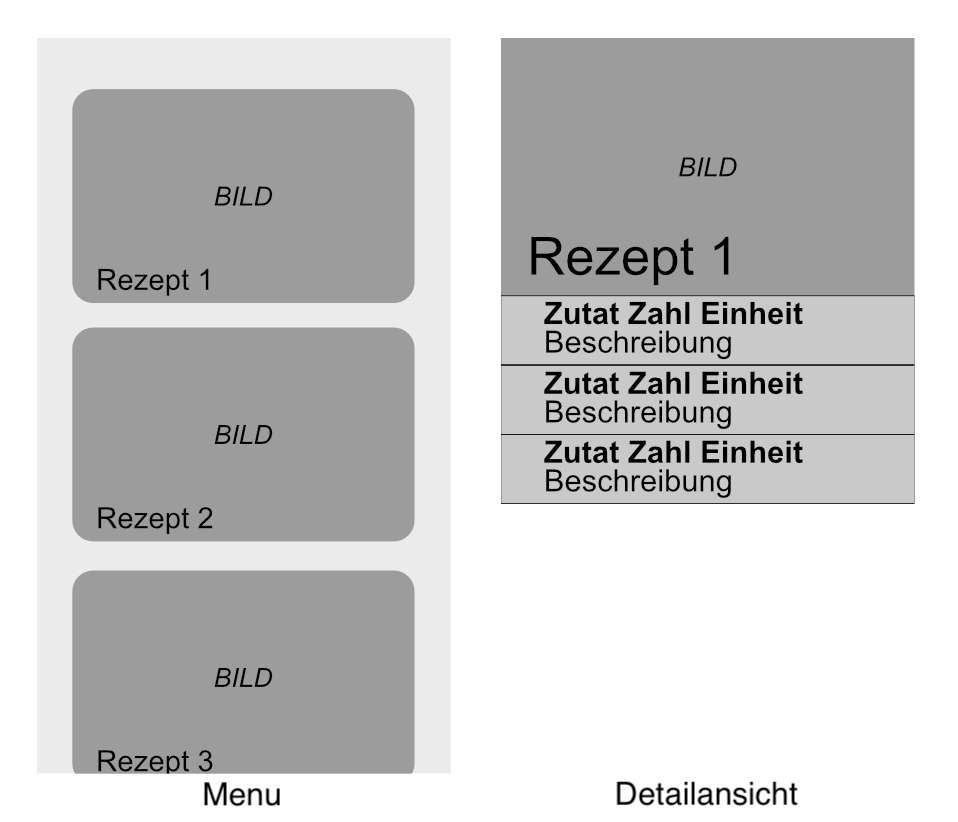
\includegraphics[width=\linewidth]{pictures/Sketch.png}
    \caption{Frühe Skizze}
    \label{fig:earlySketch}
\end{figure}

\section{Fazit}
Text.

\bibliographystyle{unsrt}
\renewcommand\refname{Bibliografie}
\bibliography{main}

\end{document}